\documentclass{beamer}
\usepackage[utf8x]{inputenc}
\usepackage[french]{babel} 
\usepackage{lmodern}
\usepackage[T1]{fontenc}
\usepackage{graphicx}
\usetheme{Hannover}
\title[Phishing-Wlan]{Network 101\\Phishing-wlan}
\author{Authors}
\institute{Institute}
\date{September 21, 2015}
\begin{document}

\begin{frame}
	\titlepage
\end{frame}

\AtBeginSubsection[]
{
	\begin{frame}<beamer>
		\frametitle{Layout}
		\tableofcontents[currentsection,currentsubsection]
	\end{frame}
}

\section{Introduction}
\begin{frame}{Introduction}
	Introduction\\
	This project can be sum up by several steps :\\
	\begin{itemize}
		\pause \item Scan the Network and choose a victim\\
		\pause \item Setup a MITM Attack on the Local Area Network\\
			\begin{itemize}
    			\pause \item ARP Spoofing\\
    			\pause \item DNS Spoofing\\
    			\pause \item steal SSL certificate\\
    		\end{itemize}
		\pause \item Steal credentials\\
	\end{itemize}
\end{frame}

\section{What we are doing}
\subsection{Global Process}
\begin{frame}{Global Process}
	\begin{figure}[!h]
		\centering
		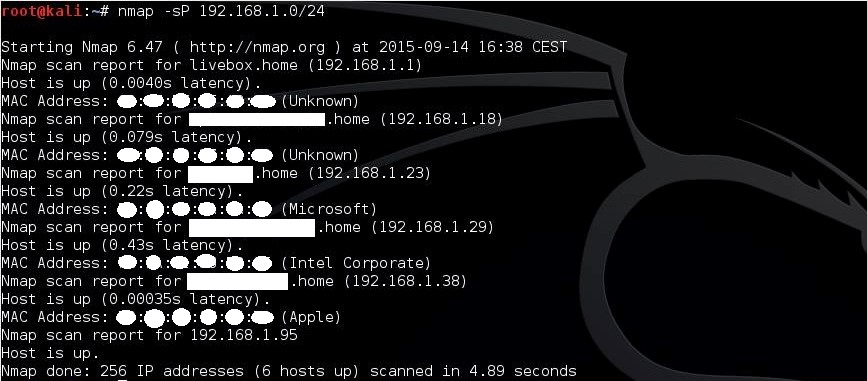
\includegraphics[scale=0.45]{../images/captureNMAP.jpg}
		\caption{nmap capture}
		\label{nmap_capture}
	\end{figure}
\end{frame}

\subsubsection{ARP Step}
\begin{frame}{ARP Step}
	\begin{figure}[!h]
		\centering
		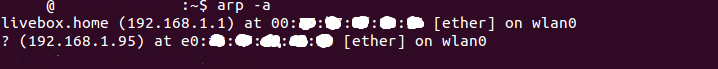
\includegraphics[scale=0.50]{../images/arpTableBeforeSpoof.png}
		\caption{ARP Table before spoof}
		\label{ARP_before_spoof}
	\end{figure}
	\begin{figure}[!h]
		\centering
		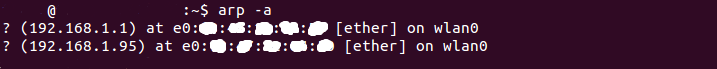
\includegraphics[scale=0.50]{../images/arpTableAfterSpoof.png}
		\caption{ARP Table after spoof}
		\label{ARP_after_spoof}
	\end{figure}	
\end{frame}

\begin{frame}{ARP spoof message}
	%\begin{center}
		%\begin{verbatim}
			%<MAC_PIRATE> tell <MAC_TARGET> that <IP_GATEWAY> is at <MAC_PIRATE>
		%\end{verbatim}
	%\end{center}

	\begin{figure}[!h]
		\centering
		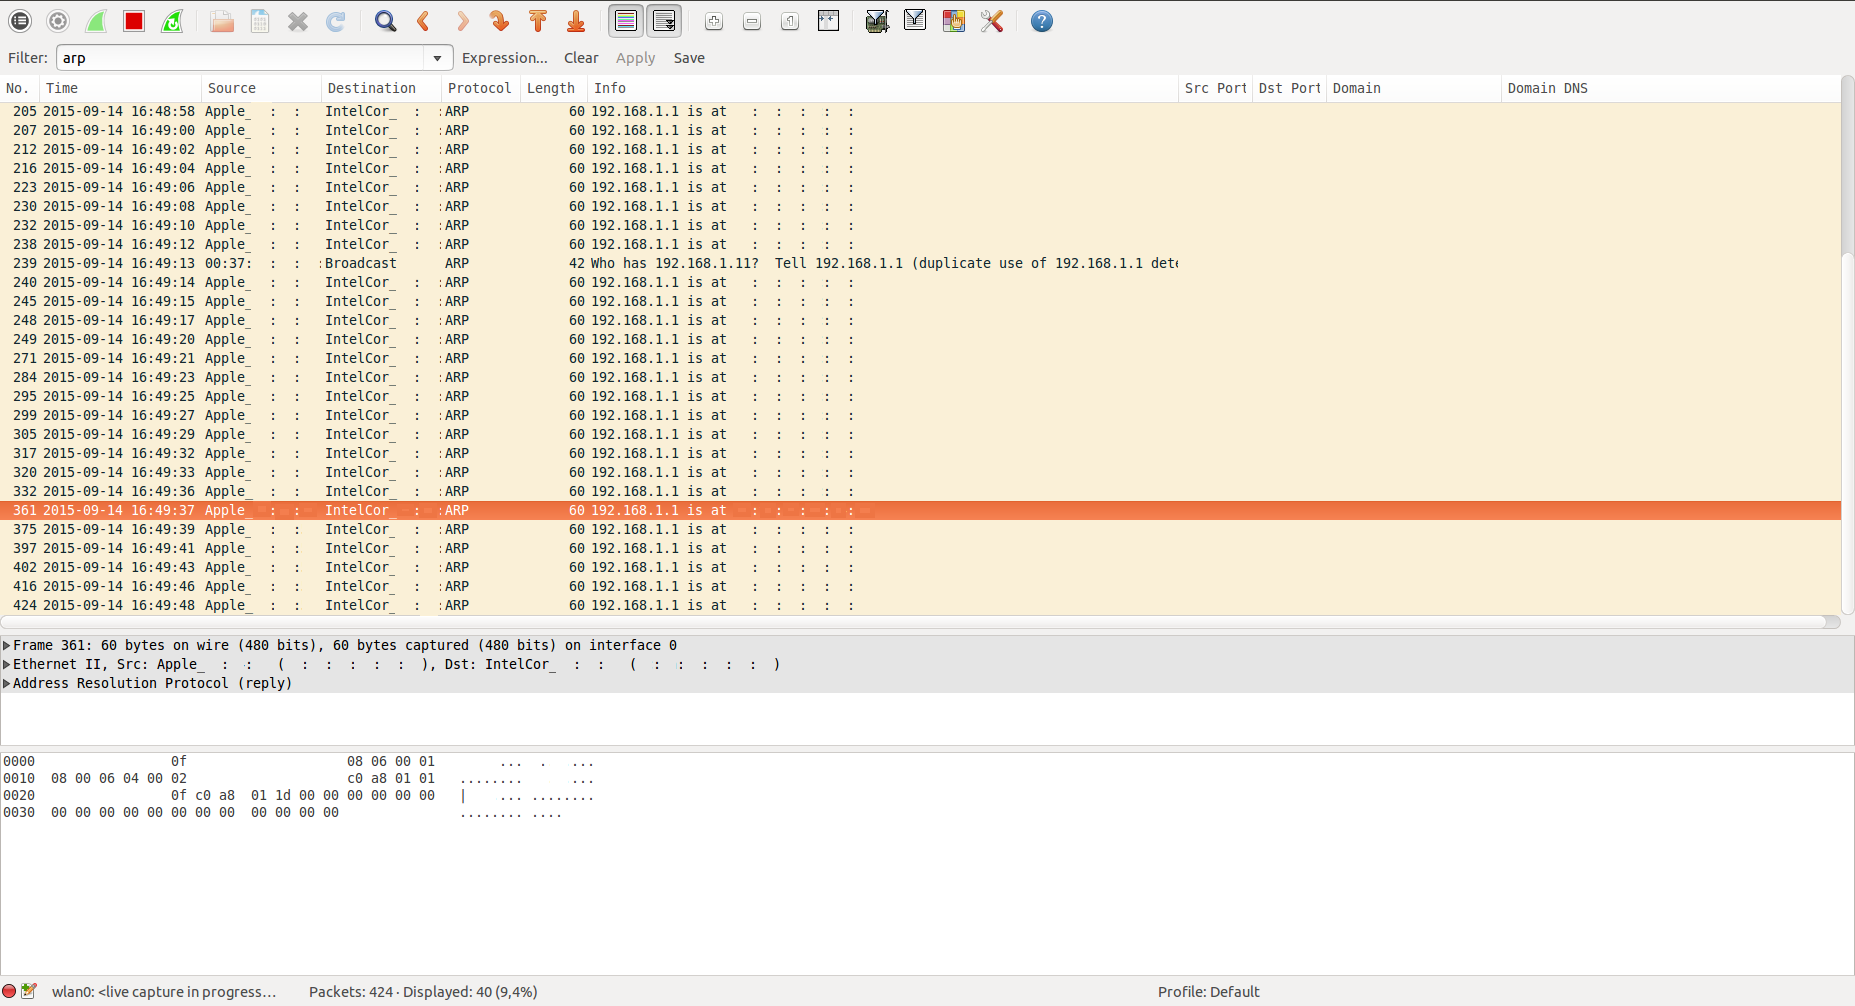
\includegraphics[scale=0.2]{../images/wiresharArpSpoof.png}
		\caption{Wireshark capture of the ARP spoofing}
		\label{Wireshark_ARP_Spoof}
	\end{figure}
\end{frame}

\subsubsection{DNS Step}
\begin{frame}{DNS Step}
	\begin{figure}[!h]
		\centering
		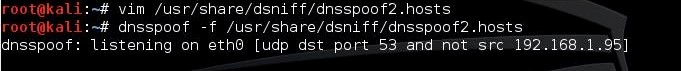
\includegraphics[scale=0.50]{../images/dnsSpoof.jpg}
		\caption{DNS spoofing}
		\label{DNS_spoofing}
	\end{figure}
\end{frame}

\subsubsection{HTTP Server Step}
\begin{frame}{HTTP Server Step}
	\begin{figure}[!h]
		\centering
		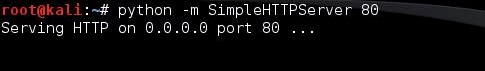
\includegraphics[scale=0.75]{../images/serverHTTP.jpg}
		\caption{HTTP server}
		\label{serverHTTP}
	\end{figure}
\end{frame}

\subsection{Legal testing}
\begin{frame}{What we did to legally test security flaw}
	\begin{itemize}
		\pause \item Work on a personnal WLAN\\
		\pause \item Every test was ran on our personnal machines\\
	\end{itemize}
\end{frame}

\subsection{Counter measures}
\begin{frame}{Counter measures to prevent this kind of attack}
For the website owner : \\
	\begin{itemize}
		\pause \item not providing an HTTP version of his website\\
		\pause \item acquire a legitimate HTTPS certificate\\
	\end{itemize}
For the internet user : \\
	\begin{itemize}
		\pause \item always browse on a secured network you trust (ie not on a public WI-FI)\\
		\pause \item always browse on a HTTPS website with trusted and verified certificate\\
	\end{itemize}
\end{frame}

\section{Encountered problems}

\subsection{What they were}
\begin{frame}{What they were}

\end{frame}

\subsection{How we actually dealt with them}
\begin{frame}{How we actually dealt with them}

\end{frame}

\section{Differences with the Overview's Objectives}
\subsection{What are those differences (if any)?}
\begin{frame}{What are those differences (if any)?}

\end{frame}

\end{document}